\documentclass[11pt]{article}
\usepackage{amsmath,amssymb}
\usepackage{graphicx}
\usepackage{array}
\usepackage{changes}
\usepackage{natbib}
\graphicspath{ {/Users/kennedy/Desktop} }
\usepackage[margin=1in]{geometry}
\usepackage[margin=1cm]{caption}
\usepackage[parfill]{parskip}  
\usepackage{gensymb}
\title{Notes on this SPAC implementation\large}
\author{Daniel Kennedy - djk2120@columbia.edu 
}

\begin{document}
\maketitle

\section{Introduction}
\section{Model description}

\subsection{Plant Water Supply Equations}

The basic Darcy flux is described by:

\begin{equation}
q = -\int_{\psi_{soil}}^{\psi_{leaf}}{k\left(\psi\right)d\psi}
\end{equation}

And we adopt a simple linear conductance attenuation parameterization:

\begin{equation}
k(\psi) = \dfrac{\psi - p_2}{p_1 - p_2} \cdot k_\text{max}
\end{equation}

Solve the integral and define $f_k$:

\begin{equation}
q = -k_\text{max}\cdot f_k\left(\Psi_L,\Psi_s\right) \cdot \left(\psi_L-\psi_s\right)
\end{equation}

\begin{equation}
f_k = \dfrac{\dfrac{1}{2} \left(\psi_L+\psi_s\right) - p_2}{p_1 - p_2} \in \left[0,1\right]
\end{equation}

\subsection{Plant Water Demand Equations}
\begin{equation}
T = T_\text{max}\cdot f_T
\end{equation}

\begin{equation}
f_T = \dfrac{\psi_L - p_4}{p_3 - p_4} \in \left[0,1\right]
\end{equation}

\subsection{Solution}
\begin{figure}[h]
\centering
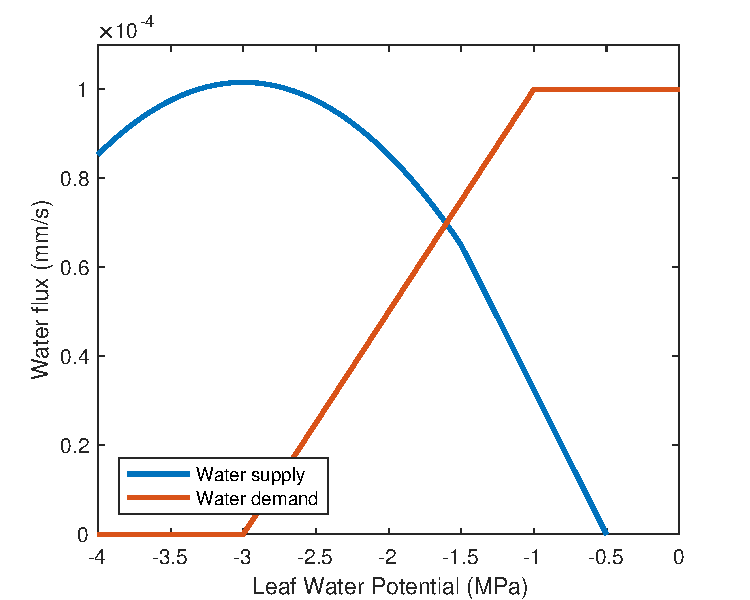
\includegraphics[width=25pc]{../figs/spac_solution}
\caption{The solution for $\Psi_L$ occurs where the two curves intersect.}
\label{fig:soln}
\end{figure}

\clearpage
\bibliographystyle{abbrvnat}
\nocite{*}

\bibliography{refs/all}





\end{document}




